\documentclass[11pt]{article}
\usepackage[utf8]{inputenc}
\usepackage[T1]{fontenc}
\usepackage{amsmath}
\usepackage{amsfonts}
\usepackage{amssymb}
\usepackage[version=4]{mhchem}
\usepackage{stmaryrd}
\usepackage{graphicx}
\usepackage[export]{adjustbox}
\graphicspath{ {./images/} }

\begin{document}
Key Observations Regarding Historical Returns of Timberland

Timber returns are quarterly returns observed from the first quarter of 2000 to the last quarter of 2021. The next exhibit provides univariate return statistics and partial autocorrelations of returns (discussed in Session 2.4, Statistical Foundations, in the lesson Covariance, Correlation, Beta, and Autocorrelation) in the top panels, and histograms of returns in the bottom panels.

\begin{center}
\begin{tabular}{lcc}
\hline
Index (Jan. 2000-Dec. 2021) & \begin{tabular}{c}
NCREIF \\
Timber \\
\end{tabular} & \begin{tabular}{c}
MSCI World \\
Equity \\
\end{tabular} \\
\hline
Annualized Arithmetic Mean & $5.8 \%$ & $6.8 \%$ \\
Annualized Standard Deviation & $4.7 \%$ & $15.4 \%$ \\
Annualized Semivolatility & $2.5 \%$ & $11.8 \%$ \\
Annualized Median & $3.6 \%$ & $15.1 \%$ \\
Skewness & 1.3 & -0.6 \\
Excess Kurtosis & 6.5 & 1.6 \\
Sharpe Ratio & 0.7 & 0.3 \\
Sortino Ratio & 1.3 & 0.4 \\
Annualized Geometric mean & $5.7 \%$ & $5.6 \%$ \\
First-Order Autocorrelation & 0.24 & 0.1 \\
Annualized Standard Deviation & $6.1 \%$ & $17.0 \%$ \\
(Adjusted for Autocorrelation) & $12.0 \%$ & $12.8 \%$ \\
Maximum & $-6.5 \%$ & $-19.0 \%$ \\
Minimum & $-6.5 \%$ & $-54.0 \%$ \\
Max Drawdown &  &  \\
\hline
 &  &  \\
\hline
Index (Jan. 2000-Dec. 2021) & NCREIF & MSCI World \\
\hline
Annualized Arithmetic Mean & $11.4 \%$ & $6.8 \%$ \\
Annualized Standard Deviation & $6.7 \%$ & $15.4 \%$ \\
Annualized Semivolatility & $1.3 \%$ & $11.8 \%$ \\
Annualized Median & $6.9 \%$ & $15.1 \%$ \\
Skewness & 3.4 & -0.6 \\
Excess Kurtosis & 15.4 & 1.6 \\
Sharpe Ratio & 1.3 & 0.3 \\
Sortino Ratio & 6.6 & 0.4 \\
Annualized Geometric mean & $11.1 \%$ & $5.6 \%$ \\
First-Order Autocorrelation & $3.6 \%$ & 0.1 \\
Annualized Standard Deviation & $7.0 \%$ & $17.0 \%$ \\
(Adjusted for Autocorrelation) & $22.8 \%$ & $12.8 \%$ \\
Maximum & $-0.1 \%$ & $-19.0 \%$ \\
Minimum & $-0.1 \%$ & $-54.0 \%$ \\
Max Drawdown &  &  \\
\hline
\end{tabular}
\end{center}

\begin{center}
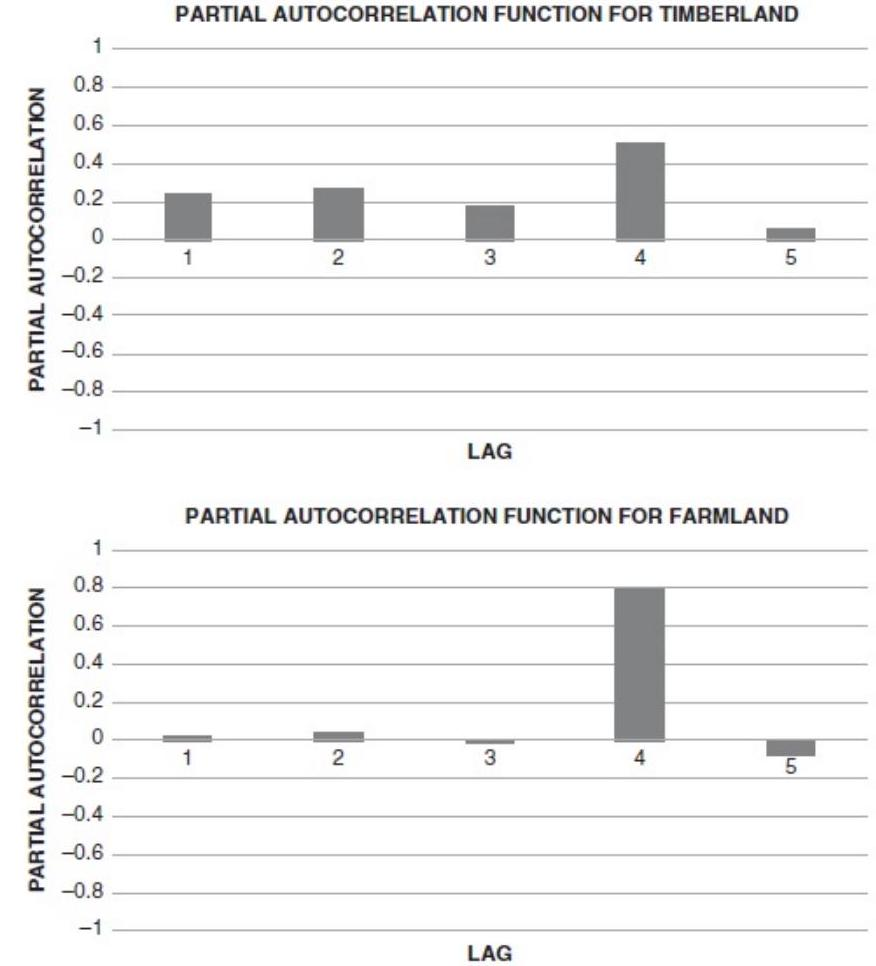
\includegraphics[max width=\textwidth]{2024_04_10_b4591cb000ecad44f255g-3(1)}
\end{center}

Histogram of Timberland Returns (Quarterly) Jan. 2000-Dec. 2021

Bucket 1: -Infinity\% $1 x<-6.0 \%$\\
Bucket 2: $-5.9 \%<x<-4.7 \%$\\
Bucket 3: $-4.6 \%<x<-3.5 \%$\\
Bucket 4: $-3.4 \%<x<-2.2 \%$\\
Bucket 5: $-2.1 \%<x<-0.9 \%$\\
Bucket 6: $-0.8 \%<x<0.3 \%$\\
Bucket 7: $0.4 \%<x<2.8 \%$\\
Bucket 8: $2.9 \%<x<4.0 \%$\\
Bucket 9: $4.1 \%<x<5.3 \%$\\
Bucket 10: 5.4\% $2 x<6.5 \%$\\
Bucket 11: $6.6 \%<x<7.8 \%$\\
Bucket 12: $7.9 \%<x<9.0 \%$\\
Bucket 13: 9.1\% $2 x<$ Infinity \%

\begin{center}
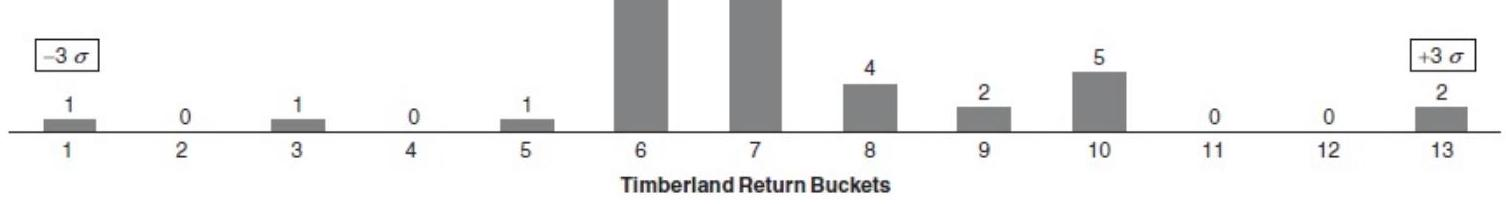
\includegraphics[max width=\textwidth]{2024_04_10_b4591cb000ecad44f255g-3}
\end{center}

Histogram of Farmland Returns (Quarterly) Jan. 2000-Dec. 2021

Bucket 1: -Infinity $\%<x<-7.5 \%$

Bucket 2: $-7.4 \%<x<-5.7 \%$

Bucket 3: $-5.6 \%<x<-4.0 \%$

Bucket 4: $-3.9 \%<x<-2.2 \%$

Bucket 5: $-2.1 \%<x<-0.4 \%$

Bucket 6: $-0.3 \%<x<1.3 \%$

Bucket 7: $1.4 \%<x<4.9 \%$

Bucket 8: $5.0 \%<x<6.6 \%$

Bucket 9: $6.7 \%<x<8.4 \%$

Bucket 10: $8.5 \%<x<10.1 \%$

Bucket 11: $10.2 \%<x<11.9 \%$

Bucket 12: $12.0 \%<x<13.7 \%$

Bucket 13: $13.8 \%<x<$ Infinity $\%$

Farmland Return Buckets

\section*{Statistical Summary of Returns}
Key observations on timber returns that are consistent with economic reasoning (and are consistent with and driven by the use of appraisals for valuations) are an essential component of knowledge and include the following:

\begin{enumerate}
  \item Timber returns had low historic volatility relative to world equities.

  \item Timber returns generated an attractive Sharpe ratio of 0.7 .

  \item Timber returns had a modestly positive skew.

  \item Timber returns had a markedly positive excess kurtosis.

  \item Timber returns enjoyed a very mild maximum drawdown (i.e., only $-6.5 \%$ ).

  \item Timber returns had a markedly high fourth-order partial autocorrelation, indicating a large one-year lag in recognizing changes in value.

  \item Timber returns were very tightly clustered around their mean.

\end{enumerate}

\end{document}